%%% Local Variables:
%%% mode: latex
%%% TeX-master: "../frankfurt"
%%% End:


\subsection{}
\begin{frame}
  \frametitle{A Parallel Implementation}

\only<2>{

\begin{greenblock}{Karger's Algorithm:}
      \begin{algorithm}[H]
        \small
        COMPACT(G, L, $k$)\\
        \KwData{A graph G, list of edges L, and parameter $k$}
\eIf{G has k vertices or $L$ = $\phi$}{
return G
   }{
     Let $L_1$ and $L_2$ be the first and second half of $L$\\
     \eIf{$H$ has fewer connected components in graph $H = (V, L_1)$}{
       return COMPACT($G$, $L$, $k$)
     }{
       return COMPACT($G\backslash L_1$, $L_2\backslash L_1$, $k$).
     }
 }

      \end{algorithm}
    \end{greenblock}

}

\only<1>{
  \begin{block}{Compact Method}
    \begin{itemize}
      \item Generating Permutations of Edges
      \item Binary searching the prefix that connects all nodes to two
        connected parts
%    \item Contraction algorithm can be implemented at
   %   $O(m\log^{\sigma}{m})$

    \item
    \end{itemize}


  \end{block}


}


\only<3>{
  \begin{figure}[!ht]
    \centering

  \end{figure}
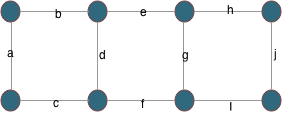
\includegraphics[scale=0.7]{img/paral.png}
}
\only<4>{
\begin{figure}[!ht]
    \centering

  \end{figure}
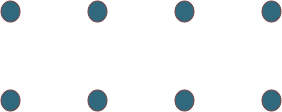
\includegraphics[scale=0.7]{img/paral1.png}
}
\only<5>{
\begin{figure}[!ht]
    \centering
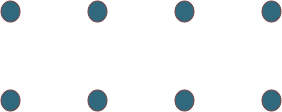
\includegraphics[scale=0.6]{img/p1.png}
  \end{figure}




\includegraphics[scale=0.7]{img/pp1.png}
}
\only<6>{
\begin{figure}[!ht]
    \centering
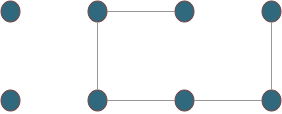
\includegraphics[scale=0.6]{img/p2.png}
  \end{figure}




\includegraphics[scale=0.7]{img/pp2.png}
}
\only<7>{
\begin{figure}[!ht]
    \centering
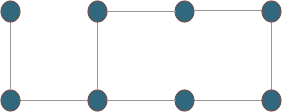
\includegraphics[scale=0.6]{img/p3.png}
  \end{figure}




\includegraphics[scale=0.7]{img/pp3.png}
}
\only<8>{
\begin{figure}[!ht]
    \centering
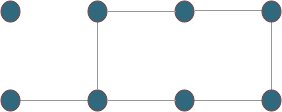
\includegraphics[scale=0.6]{img/p4.png}
  \end{figure}




\includegraphics[scale=0.7]{img/pp4.png}
}

\end{frame}
